\let\negmedspace\undefined
\let\negthickspace\undefined
\documentclass[journal]{IEEEtran}
\usepackage[a5paper, margin=10mm, onecolumn]{geometry}
%\usepackage{lmodern} % Uncomment if needed for pdflatex
\usepackage{tfrupee} % Include tfrupee package

\setlength{\headheight}{1cm} % Set the height of the header box
\setlength{\headsep}{0mm}     % Set the distance between the header box and the top of the text

\usepackage{gvv-book}
\usepackage{gvv}
\usepackage{cite}
\usepackage{amsmath,amssymb,amsfonts,amsthm}
\usepackage{algorithmic}
\usepackage{graphicx}
\usepackage{textcomp}
\usepackage{xcolor}
\usepackage{txfonts}
\usepackage{listings}
\usepackage{enumitem}
\usepackage{mathtools}
\usepackage{gensymb}
\usepackage{comment}
\usepackage[breaklinks=true]{hyperref}
\usepackage{tkz-euclide} 
\usepackage{listings}
%\usepackage{gvv}                                        
\def\inputGnumericTable{}                                 
\usepackage[latin1]{inputenc}                                
\usepackage{color}                                            
\usepackage{array}                                            
\usepackage{longtable}                                       
\usepackage{calc}                                             
\usepackage{multirow}                                         
\usepackage{hhline}                                           
\usepackage{ifthen}                                           
\usepackage{lscape}
\usepackage{tikz}
\usepackage{circuitikz}
\usepackage{standalone} % For including external TikZ files

\begin{document}

\bibliographystyle{IEEEtran}
\vspace{3cm}

\title{10.4.1.2.4}
\author{EE24BTECH11066 - YERRA AKHILESH}
% \maketitle
% \newpage
% \bigskip
{\let\newpage\relax\maketitle}

\renewcommand{\thefigure}{\theenumi}
\renewcommand{\thetable}{\theenumi}
\setlength{\intextsep}{10pt} % Space between text and floats

\numberwithin{equation}{enumi}
\numberwithin{figure}{enumi}
\renewcommand{\thetable}{\theenumi}
\textbf{Question}:\\

A train travels a distance of $480 $ km at a uniform speed. If the speed had been $8$ km/h less, then it would have taken 3 hours more to cover the same distance. We need to find the speed of the train.\\

\textbf{Solution : }\\

To solve the problem, let the speed of the train be $x$ km/h. The given conditions are :\\

-The train travels $480$ km at uniform speed $x$.\\
-If the speed is reduced by $8$ km/h i.e $\brak{x-8}$, the train would take 3 hours more to cover the same distance.\\

Time taken at speed $x$ is,
\begin{align}
    t_1 = \frac{480}{x}
\end{align}
Time taken at speed $x-8$ is,
\begin{align}
    t_2 = \frac{480}{x-8}
\end{align}
using given conditions,
\begin{align}
    t_2 - t_1 = 3\\
    \frac{480}{x-8} - \frac{480}{x} = 3
\end{align}
on simplifying,
\begin{align}
    \frac{480x - 480\brak{x-8}}{x\brak{x-8}} = 3\\
    480 \cdot 8 = 3x\brak{x-8}\\
    3x^2 -24x -3840 = 0\\
    x^2 - 8x -1280 = 0
\end{align}
We can solve the above equation using fixed point iterations. First we separate $x$, from the above equation and make an update equation of the below sort.
\begin{align}
	x = g\brak{x} \implies x_{n+1} = g\brak{x_n}
\end{align}
Applying the above update equation on our equation, we get
\begin{align}
	x_{n+1} = 	\frac{x_n^2 - 1280}{8}
\end{align}
Now we take an initial value $x_0$ and iterate the above update equation. But we realize that the updated values always approach infinity for any initial value. \\
Thus we will alternatively use \textbf{Newton's Method} for solving equations.
\begin{align}
	x_{n+1} = x_n - \frac{f\brak{x_n}}{f^{\prime}\brak{x_n}} 
\end{align}
Where we define $f\brak{x}$ as, 
\begin{align}
	f\brak{x} = x^2-8x-1280 \\
	f^{\prime}\brak{x} = 2x-8 
\end{align}
Thus, the new update equation is, 
\begin{align}
	x_{n+1} = x_n - \frac{x_n^2-8x_n-1280}{2x_n-8 } 
\end{align}
Taking the initial guess as $x_0 = 39$, we can see that $x_n$ converges with x as,
\begin{align}
	x = 40.014285714 \approx 40
\end{align}
Alternatively, we can use the Secant method for solving equations.
\begin{align}
	x_{n+1} = x_n + f\brak{x_n}\frac{x_{n} -  x_{n-1}}{f(x_{n}) -  f(x_{n-1})}
\end{align}
Newton's method is very powerful but has the disadvantage that the derivative may sometimes be a far more difficult expression than \(f(x)\) itself and its evaluation therefore it may be more computationally expensive. The secant's method is more computationally cheap as the equation of the derivative is avoided by taking 2 starting points.\\ 


Using \textbf{Eigen value} approach:
\subsection*{Matrix-Based Method}
For a polynomial equation of the form:
\begin{align}
    x^n + b_{n-1}x^{n-1} + \cdots + b_2x^2 + b_1x + b_0 = 0
\end{align}
we construct a matrix called the \textit{companion matrix}, which is defined as:
\begin{align}
    \Lambda =
    \begin{bmatrix}
        0 & 1 & 0 & \cdots & 0 \\
        0 & 0 & 1 & \cdots & 0 \\
        \vdots & \vdots & \vdots & \ddots & \vdots \\
        0 & 0 & 0 & \cdots & 1 \\
        -b_0 & -b_1 & -b_2 & \cdots & -b_{n-1}
    \end{bmatrix}
\end{align}

The eigenvalues of this matrix are the roots of the given polynomial equation.

For the quadratic equation $x^2 - 8x - 1280 = 0 $, we can write it as:
\begin{align}
    x^2 + (-8)x + (-1280) = 0
\end{align}
The coefficients are:
\begin{align}
    b_1 = -8, \quad b_0 = -1280
\end{align}
The companion matrix for this equation is:
\begin{align}
    \Lambda =
    \begin{bmatrix}
        0 & 1 \\
        -(-1280) & -(-8)
    \end{bmatrix}
    =
    \begin{bmatrix}
        0 & 1 \\
        1280 & 8
    \end{bmatrix}
\end{align}
\subsection*{Eigenvalue Computation}
The eigenvalues of \( \Lambda \) are obtained by solving:
\begin{align}
    \det(\Lambda - \lambda I) = 0
\end{align}
Substitute \( \Lambda \):
\begin{align}
    \begin{vmatrix}
        0 - \lambda & 1 \\
        1280 & 8 - \lambda
    \end{vmatrix}
    = 0
\end{align}
Simplify the determinant:
\begin{align}
    (-\lambda)(8 - \lambda) - (1280)(1) = 0 \\
    \lambda^2 - 8\lambda - 1280 = 0
\end{align}
This is the original quadratic equation, so the eigenvalues are the roots itself:
\begin{align}
    \lambda_1 = 40, \quad \lambda_2 = -32
\end{align}
\section*{QR Algorithm for Finding Eigenvalues and Roots of a Quadratic Equation}

Consider the quadratic equation:
\[
x^2 - 8x - 1280 = 0
\]
We aim to find its roots using the QR algorithm, which finds the eigenvalues of the companion matrix of the quadratic polynomial.

\subsection*{1. Companion Matrix of the Polynomial}
The companion matrix \( \Lambda \) of the polynomial \( x^2 - 8x - 1280 \) is given by:
\[
\Lambda 
= \begin{pmatrix}
0 & 1 \\
1280 & 8
\end{pmatrix}
\]
This matrix represents the system that corresponds to the given polynomial.
\subsection*{2. QR Decomposition}
The QR algorithm starts by performing QR decomposition on the matrix \( \Lambda \). The goal is to decompose \( \Lambda \) into an orthogonal matrix \( Q \) and an upper triangular matrix \( R \), such that:
\[
\Lambda = QR
\]
where \( Q^T Q = I \), and \( R \) is upper triangular. Then, we form a new matrix \( \Lambda' \) as:
\[
\Lambda' = RQ
\]
This process is repeated iteratively until \( \Lambda' \) converges to an upper triangular matrix whose diagonal elements are the eigenvalues of \( \Lambda \), which correspond to the roots of the quadratic equation.

\subsection*{3. Iterative Process}
Let's outline the iterative steps for the QR algorithm applied to this companion matrix.

\subsubsection*{First Iteration:}
We start with \( \Lambda_0 = \begin{pmatrix} 0 & 1 \\ 1280 & 8 \end{pmatrix} \).

Perform the QR decomposition of \( \Lambda_0 \):
\[
\Lambda_0 = QR
\]
Let's calculate \( Q \) and \( R \), then form \( \Lambda_1 = RQ \).

\subsubsection*{Subsequent Iterations:}
Repeat the QR decomposition on the new matrix \( \Lambda_1 \), then form \( \Lambda_2 = RQ \), and so on, until the matrix \( \Lambda_k \) converges to an upper triangular form. The diagonal elements of this matrix represent the eigenvalues of \( \Lambda_0 \), which are the roots of the quadratic equation.

\subsection*{4. Eigenvalues and Roots}
After sufficient iterations, the QR algorithm will converge to an upper triangular matrix where the diagonal entries are the eigenvalues. These eigenvalues correspond to the roots of the polynomial. In this case, the eigenvalues of the companion matrix \( \Lambda \) will give us the roots of the quadratic equation \( x^2 - 8x - 1280 = 0 \).

Thus, the eigenvalues (roots) are the solutions to the quadratic equation:
\[
x = \frac{8 \pm \sqrt{8^2 - 4(1)(-1280)}}{2(1)} = \frac{8 \pm \sqrt{64 + 5120}}{2} = \frac{8 \pm \sqrt{5184}}{2}
\]
\[
x = \frac{8 \pm 72}{2}
\]
Hence, the roots are:
\[
x_1 = 40, \quad x_2 = -32
\]
As we have to find out the speed of train so, I took a positive value i.e $40$ km/h and this root is plotted below:
\begin{figure}[!ht]
		\centering
		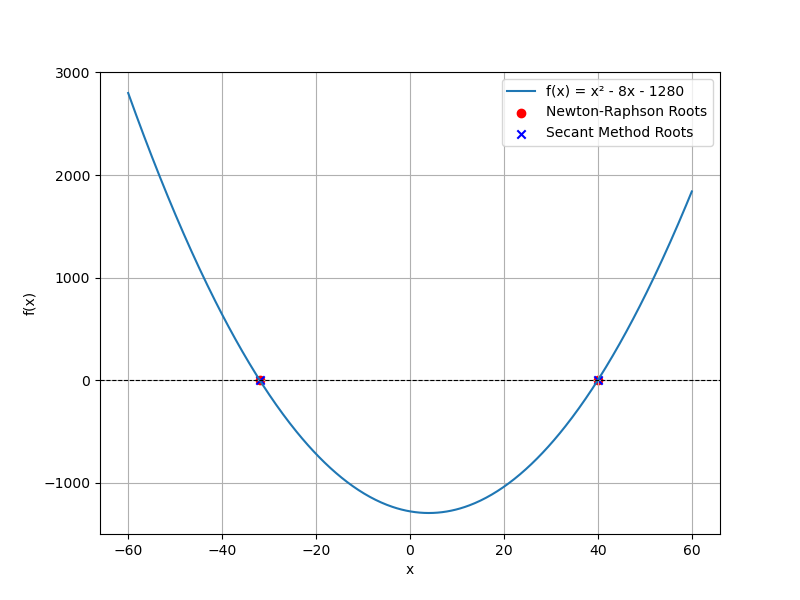
\includegraphics[width=\columnwidth]{figs/Figure_1.png}
		\caption{Solution of the given function}
		\label{stemplot}
	\end{figure}
\end{document}
